\documentclass{article}
\usepackage{fancyhdr} % for pretty formatting
\usepackage{amsmath} % for matrices
\usepackage{amssymb} % for bold text
\usepackage{pgfplots} % for graphs
\usepackage{hyperref} % for hyperlinks
\pgfplotsset{compat=1.18}
\usepackage{enumitem} % for custom lists

\usepackage{tikz}
\usepackage[svgnames]{xcolor}

\usepackage{lipsum} % For dummy text
\usepackage{cite} % For citations

\pagestyle{fancy}  
\fancyhf{} % Clear all header and footer fields

\usepackage{tcolorbox} % Required for tcolorbox

\newtcolorbox{solutioncheck}{
    colback=green!10, % Background color
    colframe=gray!50, % Frame color
    boxsep=5pt, % Padding
    arc=4pt, % Rounded corners
    title=Checking solution, % Optional title for the aside
    fonttitle=\bfseries, % Title font style
} % for Asides

\lhead{Joshua Dunne}
\rhead{\thepage} % Displays the current page number 
\lfoot{MATH620}
\rfoot{Unit 4}
\cfoot{Homework 5}

\begin{document}
    \section{Question 1}


        \paragraph{Consider} 
            $$A=\begin{bmatrix}6&-2\\1&3\end{bmatrix},\enspace B=\begin{bmatrix}5&-2\\3&-7\end{bmatrix}$$
        \subsection{Parts}
    
            \begin{enumerate}[label=(\alph*)]
                \item Find $det(A)$ and $det(B)$
                    \begin{center}
                        $det(A)=(6)(3)-(1)(-2)=18+2=20$ \\
                        $det(B)=(5)(-7)-(3)(-2)=-35+6=-29$
                    \end{center}
                \item Create new matrices by interchanging columns. Find the determinant.
                      Conjecture about how the swap affected the determinant
                        \[A'=\begin{bmatrix}-2&6\\3&1\end{bmatrix},\enspace B'=\begin{bmatrix}-2&5\\-7&3\end{bmatrix}\]
                        \[det(A')=(-2)(1)-(3)(6)=-2-18=-20\]
                        \[det(B')=(-2)(3)-(5)(-7)=-6+35=29\]
                      When we transpose the columns it seems like we're flipping the sign on the determinant.
                      This is easy to double check so, let's have a look before moving on
                        \[det(A)=det\left(\begin{bmatrix}a&b\\c&d\end{bmatrix}\right)=ad-bc=-det(\begin{bmatrix}b&a\\d&c\end{bmatrix})=-(ad-bc)\]
                      The intuition holds, atleast for a 2x2 matrix.
                \item Create new matrices by interchanging rows. Find the determinant. 
                        \[A''=\begin{bmatrix}1&3\\6&-2\end{bmatrix},\enspace B''=\begin{bmatrix}3&-7\\5&-2\end{bmatrix}\]
                        \[det(A'')=(1)(-2)-(3)(6)=-2-18=-20\]
                        \[det(B'')=(3)(-2)-(-7)(5)=-6+35=29\]
                      Again. Seems we're swapping sign. To borrow from the method above
                        \[det(A)=det(\begin{bmatrix}a&b\\c&d\end{bmatrix})=ad-bc=-det(A'')=-det(\begin{bmatrix}c&d\\a&b\end{bmatrix})=-(ad-bc)\]
                      The intuition holds, atleast for a 2x2 matrix.
                \pagebreak
                \item Consider the original matrix. Draw the parallelogram formed by the matrix with interchanged rows.
                      \begin{figure}[h!]
                        \hspace{1.2cm}
                        \noindent
                        \centering
                        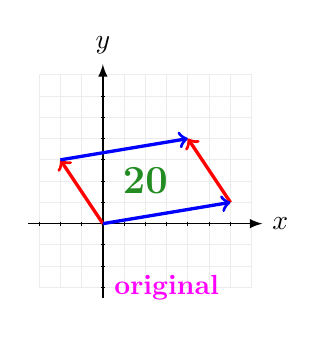
\begin{tikzpicture}
                        [
                            scale=0.27,
                            vector style/.style={->, very thick}
                        ]
                        \draw[gray!15,step=1cm] (-3,-3) grid (7,7);
                        \draw[line width=0.2mm, -latex] (-3.5,0) -- (7.5,0) node[right] {$x$};
                        \foreach \x in {-3,...,7} \draw (\x,.1)--(\x,-.1);
                        \draw[line width=0.2mm, -latex] (0,-3.5) -- (0,7.5) node[above] {$y$};
                        \foreach \y in {-3,...,7} \draw (.1,\y)--(-.1,\y);
                        \draw (0.3,0.3) node[anchor=west] {}; % Clear the (0,0) label
                        \draw[vector style, color=red, opacity=1] (0,0) -- (-2,3) node[above,,yshift=-1.5mm] {};
                        \draw[vector style, color=blue, opacity=1] (-2,3) -- (4,4) node[right,,yshift=-1.5mm] {} ;
                        \draw[vector style, color=red, opacity=1] (6,1) -- (4,4) node[right,yshift=-1.5mm] {};
                        \draw[vector style, color=blue, opacity=1] (0,0) -- (6,1) node[right,yshift=-1.5mm] {};
                        \node[font=\Large\bfseries\color{ForestGreen}] at (2,2) {20};
                        \node[font=\normalsize\bfseries\color{Magenta}] at (3,-3) {original};
                        \end{tikzpicture}
                        \hfill
                        % === GRAPH 2 ===
                        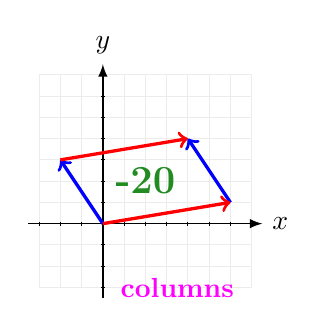
\begin{tikzpicture}
                        [
                            scale=0.27,
                            vector style/.style={->, very thick}
                        ]
                        \draw[gray!15,step=1cm] (-3,-3) grid (7,7);
                        \draw[line width=0.2mm, -latex] (-3.5,0) -- (7.5,0) node[right] {$x$};
                        \foreach \x in {-3,...,7} \draw (\x,.1)--(\x,-.1);
                        \draw[line width=0.2mm, -latex] (0,-3.5) -- (0,7.5) node[above] {$y$};
                        \foreach \y in {-3,...,7} \draw (.1,\y)--(-.1,\y);
                        \draw (0.3,0.3) node[anchor=west] {}; % Clear the (0,0) label
                        \draw[vector style, color=blue, opacity=1] (0,0) -- (-2,3) node[above,,yshift=-1.5mm] {};
                        \draw[vector style, color=red, opacity=1] (-2,3) -- (4,4) node[right,,yshift=-1.5mm] {} ;
                        \draw[vector style, color=blue, opacity=1] (6,1) -- (4,4) node[right,yshift=-1.5mm] {};
                        \draw[vector style, color=red, opacity=1] (0,0) -- (6,1) node[right,yshift=-1.5mm] {};
                        \node[font=\Large\bfseries\color{ForestGreen}] at (2,2) {-20};
                        \node[font=\normalsize\bfseries\color{Magenta}] at (3.5,-3) {columns};
                        
                        \end{tikzpicture}
                        \hfill
                        % === GRAPH 3 ===
                        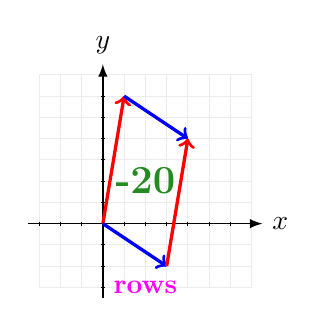
\begin{tikzpicture}
                        [
                            scale=0.27,
                            vector style/.style={->, very thick}
                        ]
                        \draw[gray!15,step=1cm] (-3,-3) grid (7,7);
                        \draw[line width=0.2mm, -latex] (-3.5,0) -- (7.5,0) node[right] {$x$};
                        \foreach \x in {-3,...,7} \draw (\x,.1)--(\x,-.1);
                        \draw[line width=0.2mm, -latex] (0,-3.5) -- (0,7.5) node[above] {$y$};
                        \foreach \y in {-3,...,7} \draw (.1,\y)--(-.1,\y);
                        \draw (0.3,0.3) node[anchor=west] {}; % Clear the (0,0) label
                        \draw[vector style, color=red, opacity=1] (0,0) -- (1,6) node[above,,yshift=-1.5mm] {};
                        \draw[vector style, color=blue, opacity=1] (0,0) -- (3,-2) node[right,,yshift=-1.5mm] {} ;
                        \draw[vector style, color=red, opacity=1] (3,-2) -- (4,4) node[right,yshift=-1.5mm] {};
                        \draw[vector style, color=blue, opacity=1] (1,6) -- (4,4) node[right,yshift=-1.5mm] {};
                        \node[font=\Large\bfseries\color{ForestGreen}] at (2,2) {-20};
                        \node[font=\normalsize\bfseries\color{Magenta}] at (2,-3) {rows};
                        \end{tikzpicture}  
                    \end{figure}
                    \footnote{Totally borrowing from Jack}
                    
                      \paragraph{Basis vectors}
                        We're keeping colors here so that the changes make some sense.
                        From this too, we're quite easily able to see that interchanging either
                        will cause us to form the parallelogram based on new basis vectors.
                        If we changed columns, we still have the same ${c_1,c_2,\dots,c_n}$
                        they're just disordered. Differently, if we interchange rows,
                        we get a different set of constants with we span.
                      \paragraph{Determinant}
                        As was demonstrated above, we flip the sign of the determinant.
                        It's\dots the same shape, it has the same area, but, as we've changed
                        the orientation of the basis vectors, we're now getting negative determinants.
            \end{enumerate}
    \section{Question 2}
      \paragraph{Given}
        \[
        C=\begin{bmatrix}1&2&3\\2&4&6\\8&9&-1\end{bmatrix}
        \,
        D=\begin{bmatrix}0&0&0\\5&-1&6\\9&2&4\end{bmatrix}
        \]
      \paragraph{Wanted}
        We want two properties of the determinant that we can gleam from the given.
      \paragraph{Linear multiple row}
          Looking at $C$ we can see that we don't seem to have dependent columns,
          but we do have linearly dependent rows as
          $$2C_{1,j}=C_{2,j}\enspace\forall{j} \in \{1,2,\dots,n\}$$
.       \subparagraph{Calulcating the determinant}
          \begin{align*}
            det(C)&=3(18-32)-2(-2)(48)+(1)(-4)(54)=0
          \end{align*}
        \subparagraph{Property}
          We can say that in this example atleast, that the existence of
          atleast one row being a linear multiple might have caused the determinant to be $0$
      \paragraph{Row of all 0}
          Looking now at $D$ we can see something even more obvious.
          Even though this still simply follows from rows being linear multiples, it'd
          \begin{align*}
            det(D)&=(0)(10+9)-\dots=0
          \end{align*}
        \subparagraph{Property}
          If we have a row of all zero's we will have a determinant of 0.
          I could flesh this out, but, we can easily brain check quickly as,
          while taking the determinant, no matter which row for a 2x2 or 3x3,
          one of the terms we're multiplying by will be 0 for each term.
  \section{Question 3}
    \begin{enumerate}[label=(\alph*)]
      \item Is $det(AB)=det(A)det(B)$? \\
        Yes. I read through the proof online, pretty sure I'm following along.
      \item What is the relationship between $A$ and $A^{-1}$?
        \[det(A)=1/det(A^{-1})\]
        The proof here is much simpler. I'm satisfied to say that, ofcourse it would be,
        we'd need the area of the parallelogram to return to it's original state.
    \end{enumerate}
  \section{Question 4}
    Oh. God. I'd forgotten this was here. Alright\dots given\dots
    \subsection{Givens}
      \begin{center}
      \begin{tabular}{ccc}
        $A=\begin{bmatrix}5&8\\-2&3\end{bmatrix}$
         & $B=\begin{bmatrix}5\alpha&8\\-2\alpha&3\end{bmatrix}$
         & $C=\begin{bmatrix}6\alpha&8\alpha\\-2\alpha&3\end{bmatrix}$
        \\[0.5cm]
        $\bar{A}=\begin{bmatrix}3&5&1\\-2&4&7\\1&2&8\end{bmatrix}$
         & $\bar{B}=\begin{bmatrix}3\alpha&5&1\\-2\alpha&4&7\\\alpha&2&8\end{bmatrix}$
         & $\bar{C}=\begin{bmatrix}3\alpha&5\alpha&\alpha\\-2\alpha&4\alpha&7\\\alpha&2\alpha&8\alpha\end{bmatrix}$
      \end{tabular}
      \end{center}
    \subsection{Sections}
    \begin{enumerate}[label=(\alph*)]
      \item Find $det(A)$ and $det(B)$
            \begin{align*}
              det(A)&=(5)(3)-(-2)(8)=15-16=-1 \\
              det(\bar{A})&=1(-4)(4)-5(-16)(7)+3(32)(14)=161
            \end{align*}
      \item Find $det(B)$ and $det(\bar{B})$
            \begin{align*}
              det(B)&=(5\alpha)(3)-(-2\alpha)(8)=15\alpha+16\alpha=31\alpha \\
              det(\bar{B})&=(-4\alpha-4\alpha)-5(-16\alpha-7\alpha)+3\alpha(32)(14)=161\alpha
            \end{align*}
      \item Find $det(C)$ and $det(\bar{C})$
            \begin{align*}
              det(C)&=(5\alpha)(3)-(-2\alpha)(8)=15\alpha+16\alpha=31\alpha \\
              det(\bar{C})&=\alpha^{2}[(-4-4)-5(-16-7)+3(32)(14)]=16\alpha^{2}
            \end{align*}
      \item \textbf{Hypothesize}
            \newline
            If $B=A$ by multiplying a column of $A$ by a scalar $k$ then 
            \begin{center}
              $det(B)=k\,det(A)$.
            \end{center}
            If $C=A$ by multiplying every element of $A$ by a scalar $k$ then
            \begin{center}
              $det(C)=k^2\,det(A)$.
            \end{center}

    \end{enumerate}
\end{document}